\documentclass[a4paper]{article}

%% Language and font encodings
\usepackage[english]{babel}
\usepackage[utf8x]{inputenc}
\usepackage[T1]{fontenc}

%% Sets page size and margins
\usepackage[a4paper,top=3cm,bottom=2cm,left=3cm,right=3cm,marginparwidth=1.75cm]{geometry}

%% Useful packages
\usepackage{amsmath,amsthm,amssymb}
\usepackage{graphicx}
\usepackage[colorinlistoftodos]{todonotes}
\usepackage[colorlinks=true, allcolors=blue]{hyperref}
\newtheorem{theorem}{Theorem}
\newtheorem{lemma}{Lemma}
\newtheorem{remark}{Remark}
\newtheorem{example}{Example}
\newtheorem{corollary}{Corollary}




\newcommand{\dt}{\Delta t}
\newcommand{\dx}{\Delta x}
\newcommand{\te}{\theta}
\newcommand{\nul}{\nu_L(k,\theta)}
\newcommand{\nur}{\nu_R(k,\theta)}
\newcommand{\yl}{y_L(k,\theta)}
\newcommand{\yr}{y_R(k)}
\newcommand{\nplus}{\mathbb{N}^+}
\newcommand{\rr}{\mathbb{R}}
\newcommand{\Por}{P_{R,k}(y)}
\newcommand{\Pol}{P_{L,k,\te}(y)}
\newcommand{\cP}{{\cal{P}}}
\newcommand{\cD}{{\cal{D}}}






\title{Positivity of implicit discretizations of the advection equation}
\author{Yiannis Hadjimichael \and David I. Ketcheson \and Lajos L\'oczi}

\begin{document}
\maketitle

\section{Background and motivation}
Here we investigate the positivity of some discretizations of the advection equation
\begin{align} \label{advection}
U_t = a U_x.
\end{align}
The advection equation is a fundamental PDE, and herein we focus on
some of the simplest and most fundamental discretizations of it.

Any linear one-step discretization of a time-dependent PDE in one spatial
dimention with $m$ grid points in space yields an approximate solution given by
an iteration of the form
where $M$ is a fixed $m\times m$ matrix.


\subsection{Discrete Fourier analysis}
Any finite difference semi-discretization of \eqref{advection} with
periodic boundary conditions yields a system of ODEs
\begin{align} \label{semi-discrete}
    u'(t) & = \frac{a}{\dx}Lu(t)
\end{align}
where $L$ is a circulant matrix, which has the eigendecomposition
\begin{align}
    L & = F \Lambda F^*
\end{align}
where the (unitary) matrix of eigenvectors has entries
\begin{align}
    f_{jk} & = \exp(i \xi_k (j-1))/\sqrt{m}  & 1 \le j, k \le m
\end{align}
and $\Lambda$ is the diagonal matrix of eigenvalues, which depends on the
particular finite difference method chosen.  Here $\xi_k$ are the
$m$th roots of unity:
\begin{align}
    \xi_k & = \frac{2\pi(k-1)}{m} & 1 \le k \le m.
\end{align}

Applying a one-step time
discretization with stability function $R(z)$ to \eqref{semi-discrete} leads to
the iteration
\begin{align} \label{M}
    u^{n+1} & = R(\nu L) u^n = Mu^n
\end{align}
where $M=F^* R(\nu \Lambda) F$ and $\nu=a\dt/\dx$ is the CFL number.  The
necessary and sufficient condition for positive invariance of the numerical
solution is then simply that every entry of $M$ be nonnegative.

Note that $M$ is also a real, circulant matrix.
Thus it is defined completely by the entries of its first row, which
are given by
\begin{align} \label{M-entries}
    M_{1,j} & = \frac{1}{m} \sum_{k=1}^m R(\nu\lambda_k) \exp(-i(j-1)\xi_k).
\end{align}

\section{Backward in time, centered in space}
Consider the case of a 3-point centered difference in space:
\begin{align}
    U_x|_{x=x_j} \approx \frac{u_{j+1}-u_{j-1}}{2\dx}
\end{align}
so that $L$ is a circulant matrix with entries $(-1/2, 0, 1/2)$ on the central
three diagonals.  The exact solution of the resulting semi-discrete
system \eqref{semi-discrete} is not positive invariant, so (given an appropriate
positive initial condition) any consistent time discretization will yield
negative values for small enough time steps.  Here we investigate whether
it is possible to ensure positive invariance for large time steps.

Let us consider first the backward Euler method.
The eigenvalues for this semi-discretization are $\lambda_j = i\sin\xi_j$.
If we use the backward Euler method in time, we have $R(z) = (1-z)^{-1}$, so
\eqref{M-entries} gives the entries of $M$ as
\begin{align} \label{firstrow}
    M_{1,j} & = \frac{1}{m} \sum_{k=1}^m \frac{\exp\left(-i(j-1)\xi_k\right)}{1-\nu i \sin\xi_k}.
\end{align}
If $m$ is even, then these entries cannot all be positive.

\begin{lemma}
    If $m$ is even, then $M_{1,m} < 0$.
\end{lemma}
\begin{proof}
    From \eqref{firstrow} we have
    \begin{align}  \label{M12}
        M_{1,m} & = \frac{1}{m} \sum_{k=1}^m \frac{ \exp(-i(m-1)\xi_k)}{1-\nu i \sin\xi_k}
                  = \frac{1}{m} \sum_{k=1}^m \frac{ \exp(i\xi_k)}{1-\nu i \sin\xi_k}
                  = \frac{1}{m} \sum_{k=1}^m \frac{\cos \xi_k - \nu \sin^2 \xi_k}{1+\nu^2 \sin^2 \xi_k}.
    \end{align}
    The expression on the right is obtained by multiplying by the complex
    conjugate of the denominator and taking the real part (since $M$ is a real matrix).
    Due to symmetry, when $m$ is even,
    \begin{align*}
        \sum_{k=1}^m \frac{\cos \xi_k}{1+\nu^2\sin^2\xi_k}  = \sum_{k=1}^{m/2} \frac{\cos \xi_k + \cos(\xi_k+\pi)}{1+\nu^2\sin^2\xi_k} = 0,
    \end{align*}
    Thus 
    \begin{align*} 
        M_{1,m} & = \frac{1}{m} \sum_{k=1}^m \frac{- \nu \sin^2 \xi_k}{1+\nu^2 \sin^2 \xi_k} < 0.
    \end{align*}
\end{proof}
Using similar expressions, it can in fact be shown that, for $m$ even, we have
$M_{1,2j}<0$ for $1\le j \le m/4$; in other words, approximately one fourth of
the entries of $M$ are negative, no matter the value of $\nu$.  All of these
negative entries tend to zero as $\nu \to \infty$.

Meanwhile, if $m$ is odd...


Next we generalize the above results to the theta method.  In this case we have
\begin{align}
    R(z) & = \frac{1+(1-\theta)z}{1-\theta z}
\end{align}
so with the centered difference in space we get
\begin{align} \label{firstrow-theta}
    M_{1,j} & = \frac{1}{m} \sum_{k=1}^m \frac{1+(1-\theta)\nu i\sin\xi_k}{1-\theta\nu i \sin\xi_k}\exp\left(-i(j-1)\xi_k\right).
\end{align}
This leads to
\begin{align*} 
    M_{1,m} & = \frac{1}{m} \sum_{k=1}^m \frac{\cos\xi_k(1-\theta(1-\theta)\nu^2\sin^2\xi_k)- \nu \sin^2 \xi_k}{1+\theta^2\nu^2 \sin^2 \xi_k}.
\end{align*}
For even $m$, the sum over the first term in the numerator vanishes due to symmetry and we have
\begin{align*}
    M_{1,m} & =  \frac{1}{m} \sum_{k=1}^m \frac{- \nu \sin^2 \xi_k}{1+\theta^2\nu^2 \sin^2 \xi_k} < 0.
\end{align*}

\begin{theorem}
Consider the backward in time, centered in space discretization of the
advection equation with periodic boundary conditions and $m$ spatial grid
points.  The discretization takes the form \eqref{M},
where (i) if $m$ is even, then $M$ has at least one negative entry;
(ii) if $m$ is odd, then for $\dt>\dt_*$ all entries of $M$ are nonnegative.

(add details about $\dt_*$)
\end{theorem}

\subsection{Discrete Fourier analysis}
David's work here.

\subsection{Explicit description of the matrix entries for odd values of $m$}\label{explsect}

The explicit forms of the matrix $M$ obtained so far are independent of the question of non-negativity, and may be applicable in other contexts as well. The main theme is low-order recursions. As we will see, these appear throughout our work.

Mention: enough to focus on the 1st row: the sum/product/inverse of circulant matrices is circulant [REFERENCE: Fact 5.16.7. in Berstein MATRIX MATHEMATICS]. Since $L$ and $I$ are circulant, the matrix $M$ is circulant, too.\\
Financial support: TKP project + KAUST

We used Wolfram \textit{Mathematica} (version 11) for the computations in this work.



Some notation \\

 We need the explicit form of $L$---the first row.\\

$M\ge 0$ means that  $M_{i,j}\ge 0$ for every entry $1\le i, j\le m$.\\

$M\not\ge 0$ means there is at least one negative entry $M_{i,j}<0$.\\



$\imath^2=-1$ 

\begin{equation}\label{Mdef}
M(m,\te,\nu):=(I-\te\nu L)^{-1}(I+(1-\te)\nu L),
\end{equation}
where $I\in\rr^{m\times m}$ is the identity matrix. The dependence of $M$ on its parameters will often be suppressed. To emphasize the dimensions of a matrix, we will sometimes write, for example, $L_{m\times m}$.




HANDLE THE TRIVIAL CASE $\te=0$ FIRST.\\

MENTION THAT $M_{1,2}=-M_{1,2k}$\\

Throughout this section we can thus assume that 
\[
\boxed{m=2k+1\quad (k\in\nplus), \ \ \ \nu>0 \text{\ \  and\ \  } 0<\te\le 1.}
\]
As an initial illustration, we present the first row of $M$ for some small values of $m$. 
\begin{example}\label{example1} For $m=2$, the first row of \eqref{Mdef} is
\[\frac{1}{{\theta ^2 \nu ^2}/{4}+1}\left(-\frac{1}{4} \theta ^2 \nu ^2+\frac{\theta  \nu ^2}{4}+1,\theta  \nu -\frac{\nu }{2}\right),\]
for $m=3$ we have
\[
\frac{1}{{3 \theta ^2 \nu ^2}/{4}+1}\left(-\frac{1}{4} \theta ^2 \nu ^2+\frac{\theta  \nu ^2}{2}+1,\frac{\theta ^2 \nu ^2}{2}-\frac{\theta  \nu ^2}{4}-\theta  \nu +\frac{\nu
   }{2},\frac{\theta ^2 \nu ^2}{2}-\frac{\theta  \nu ^2}{4}+\theta  \nu -\frac{\nu }{2}\right),
\]
and for $m=5$ one has
\[
\frac{1}{{5 \theta ^4 \nu ^4}/{16}+{5 \theta ^2 \nu ^2}/{4}+1}\left(-\frac{3}{16} \theta ^4 \nu ^4+\frac{\theta ^3 \nu^4}{4}+\frac{\theta ^2 \nu ^2}{4}+\frac{\theta  \nu ^2}{2}+1,\right.
\]
\[  
\frac{\theta ^4 \nu^4}{8}-\frac{\theta ^3 \nu ^4}{16}-\frac{\theta ^3 \nu ^3}{2}+\frac{\theta ^2 \nu ^3}{4}-\theta  \nu +\frac{\nu }{2},\frac{\theta ^4 \nu^4}{8}-\frac{\theta ^3 \nu ^4}{16}+\frac{\theta ^3 \nu ^3}{4}-\frac{\theta ^2 \nu ^3}{8}+\frac{\theta ^2 \nu ^2}{2}-\frac{\theta  \nu^2}{4},
\]
\[
\left.
\frac{\theta ^4 \nu ^4}{8}-\frac{\theta ^3 \nu ^4}{16}-\frac{\theta ^3 \nu ^3}{4}+\frac{\theta ^2 \nu ^3}{8}+\frac{\theta ^2 \nu^2}{2}-\frac{\theta  \nu ^2}{4},\frac{\theta ^4 \nu ^4}{8}-\frac{\theta ^3 \nu ^4}{16}+\frac{\theta ^3 \nu ^3}{2}-\frac{\theta ^2 \nu ^3}{4}+\theta 
   \nu -\frac{\nu }{2}\right).
\]
\end{example}


Each element of $M$ is a rational function in the variables $\te$ and $\nu$. From \eqref{Mdef} it is clear that 
\[
M_{1,j}=\frac{\cP_{j,k}(\te,\nu) }{\cD_k(\te,\nu)}\quad\quad(j=1,2,\ldots,2k+1),
\]
where $\cP_{j,k}$ and $\cD_{k}$ are certain bivariate polynomials in $\te$ and $\nu$, and 
\begin{equation}\label{dendet}
\cD_k:=\det\left(I_{(2k+1)\times(2k+1)}-\te\nu L_{(2k+1)\times(2k+1)}\right).
\end{equation}

The key observation is that the polynomials $\cP_{j,k}$ and $\cD_{k}$ satisfy certain low-order linear recursions with constant coefficients. 

\begin{remark}
 \textit{Mathematica}'s  {\tt{FindLinearRecurrence}} command proved to be extremely useful for conjecturing and setting up these linear recursions. 
\end{remark}
At this point, as already suggested by Example \ref{example1}, it seems convenient to introduce the variable
\[
\mu:=\te^2\nu^2>0.
\]

On the one hand, as it turns out, $\cP_{1,k}$ and $\cD_{k}$ satisfy the same second-order recursion
in the variable $k$ (with different initial conditions), with characteristic polynomial 
\[
\kappa ^2-\kappa  \left(1+\frac{\mu }{2}\right)+\frac{\mu ^2}{16},
\]
where  $\kappa$  denotes the dummy variable. The roots of this polynomial are
\begin{equation}\label{kappa12}
\kappa_{1,2}=\frac{2+\mu \pm 2 \sqrt{\mu +1}}{4}=\left(\frac{\sqrt{1+\mu}\pm 1}{2}\right)^2.
\end{equation}


On the other hand, for any fixed $j=2, \ldots, 2k+1$, each polynomial $\cP_{j,k}$ satisfies the same third-order recursion in the variable $k$ (with initial conditions depending on $j$), with characteristic polynomial 
\[
\kappa ^3-\kappa ^2 \left(1+\frac{3 \mu }{4}\right)+\kappa  \left(\frac{\mu }{4}+\frac{3 \mu ^2}{16}\right)-\frac{\mu ^3}{64}=\left(\kappa-\frac{\mu }{4}\right)\left(\kappa ^2-\kappa  \left(1+\frac{\mu }{2}\right)+\frac{\mu ^2}{16}\right),
\]
hence the characteristic roots are $\kappa_{1,2}$ as in \eqref{kappa12}, and $\kappa_3={\mu }/{4}$.

Before proceeding, let us introduce yet another variable, which will further simplify our exposition by eliminating the square roots in \eqref{kappa12}. We set
\[
y:=\frac{\sqrt{1+\mu}-1}{\sqrt{\mu}}=\frac{\sqrt{1+\te^2\nu^2}-1}{\te\nu}\in (0,1).
\]
It is easily seen that the transformation
\[
(0,+\infty)\ni\mu \longleftrightarrow y\in(0,1)
\]
is bijective. Moreover, the following (inverse) relations will be useful:
\[
\mu=\left(\frac{2y}{1-y^2}\right)^2,
\]
\[\mu y^2=2+\mu-2\sqrt{1+\mu},\]
\[\mu/y^2=2+\mu+2\sqrt{1+\mu},\]
and
\[
\nu=\frac{2y}{1-y^2}\cdot\frac{1}{\te}.
\]

First we deal with the polynomials $\cD_k$. By carrying out some determinant expansions, we see that the determinants \eqref{dendet} obey the recursion
\[
\cD_{k+2}=\left(1+\frac{\mu}{2}\right)\cD_{k+1}-\frac{\mu^2}{16}\cD_k
\]
with initial conditions
\[
\cD_1=1+\frac{3\mu}{4}, \quad \cD_2=1+\frac{5\mu}{4}+\frac{5\mu^2}{16}.
\]
After solving this recursion, we obtain
\[
\cD_k=\left(\frac{\sqrt{1+\mu}+1}{2}\right)^{2 k+1}- \left(\frac{\sqrt{1+\mu}-1}{2}\right)^{2 k+1},
\]
or, in terms of the variable $y$, 
\begin{equation}\label{expldet}
\cD_k=\frac{1-y^{4 k+2}}{\left(1-y^2\right)^{2 k+1} }.
\end{equation}

Regarding the polynomials $\cP_{1,k}$, they satisfy the recursion 
\[
\cP_{1,k+2}=\left(1+\frac{\mu}{2}\right)\cP_{1,k+1}-\frac{\mu^2}{16}\cP_{1,k}
\]
with initial conditions
\[
\cP_{1,1}=1+\frac{3 \mu }{4}-\frac{\mu /\theta}{2  }, \quad \cP_{1,2}=1+\frac{5 \mu }{4}+\frac{5 \mu ^2}{16}-\frac{\mu/\theta }{2  }-\frac{\mu ^2/\theta}{4  }.
\]
From this recursion, by following the same approach as with the polynomials $\cD_k$, we derive that
\[
\cP_{1,k}=\frac{\Pol}{  \left(1+y^2\right)\left(1-y^2\right)^{2 k+1}\theta},
\] 
where the numerator is 
\[\Pol:=-\theta  y^{4 k+4}-(\theta -2) y^{4 k+2}+(\theta -2) y^2+\theta.\]
Here, the subscript $L$ abbreviates \textit{leftmost} (since $\cP_{1,k}$ appears in that position of the first row of $M$).

It is more challenging to describe the polynomials appearing in the numerator of the rational function in each matrix entry. 



Unlike in Example \ref{example1}, we will have lacunary polynomials (sparse polynomials, fewnomials)---define.\\






$\bullet$ For any $k\in\nplus$ and integer $2\le j\le 2k+1$, we define the polynomials
\[
P_{j,k}(y):=(-1)^{j-1} y^{4 k+2-j}+y^{2 k-1+j}+(-1)^j y^{2 k+1-j}+y^{j-2}.
\]
As a special case, we set
\[
\Por:=P_{2k+1,k}(y),
\]
in other words we have
\[\Por=y^{4 k}+y^{2 k+1}+y^{2 k-1}-1.\]
(Here, the subscript $R$ refers to \textit{right}.)

As a by-product, by comparing the trigonometric and algebraic representations presented above, we have obtained the following set of identities. 
\begin{corollary}
With $M$ defined in \eqref{Mdef}, $y=\frac{\sqrt{1+\te^2\nu^2}-1}{\te\nu}$, $\xi_\ell  = \frac{2\pi(\ell-1)}{2k+1}$, $\te>0$, $\nu>0$, and $k\in\nplus$, we have that
\[
M_{1,1}=\frac{\cP_{1,k}}{\cD_k}=\frac{-\theta  y^{4 k+4}-(\theta -2) y^{4 k+2}+(\theta -2) y^2+\theta}{  \left(1+y^2\right)\left(1-y^{4 k+2}\right)\theta}=
\]
\[
 \frac{1}{2k+1} \sum_{\ell=1}^{2k+1} \frac{1+\imath(1-\theta)\nu \sin(\xi_\ell)}{1-\imath\theta\nu  \sin(\xi_\ell)}.
\]
Moreover, for $j=2, 3, \ldots, 2k+1$ we have that
\[
M_{1,j}=\frac{\cP_{j,k}}{\cD_k}=\frac{\nu  \left(1-y^2\right)^2 \left((-1)^{j-1} y^{4 k+2-j}+y^{2 k-1+j}+(-1)^j y^{2 k+1-j}+y^{j-2}\right)}{2 \left(1+y^2\right) \left(1-y^{4 k+2}\right)}=
\]
\[
\frac{1}{2k+1} \sum_{\ell=1}^{2k+1} \frac{1+\imath(1-\theta)\nu \sin(\xi_\ell)}{1-\imath\theta\nu \sin(\xi_\ell)}\exp\left(-\imath(j-1)\xi_\ell\right).
\]

\end{corollary}

\subsection{Non-negativity of the matrix entries}

In this section we present a detailed description of the non-negativity properties of the matrix $M$, thanks to the explicit forms for the entries $M_{1,j}$ obtained in Section \ref{explsect}.

From \eqref{expldet} it is evident that $D(k)>0$ for any $\mu>0$ and $k\in\nplus$.

\begin{lemma}
ABOUT ITS UNIQUE ROOT.
\end{lemma}
The unique $y\in(0,1)$ for which $\Por=0$ is denoted by $\yr$. 


\begin{lemma}
ABOUT ITS UNIQUE ROOT.
\end{lemma}
The unique $y\in(0,1)$ for which $\Pol=0$ is denoted by $\yl$. 

$\bullet$ For any $k\in\nplus$ and $0<\te\le 1$ we define
\[\nur:=\frac{2\yr}{1-\yr^2}\cdot \frac{1}{\te}.\]

$\bullet$ For any $k\in\nplus$ and $0<\te\le 1$ we define
\[\nul:=\begin{cases}
 \frac{2\yl}{1-\yl^2}\cdot \frac{1}{\te} & \text{for } 0<\te<\frac{2k}{2k+1}\\
 +\infty & \text{for } \frac{2k}{2k+1}\le \te<1.
\end{cases}\]
The value $+\infty$ is introduced for convenience so as to make our later descriptions shorter.



\begin{figure}
\begin{center}
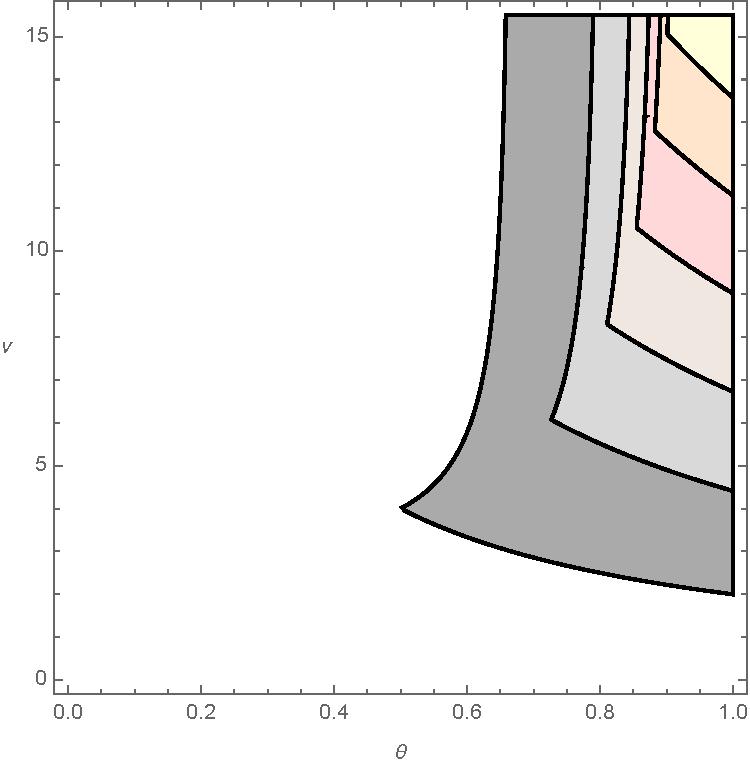
\includegraphics[width=0.48\textwidth]{fig_variousk.pdf}
\caption{The set of parameters ensuring $M(2k+1,\te,\nu)\ge 0$ in the $(\te,\nu)$ parameter plane for $k=1, 2, \ldots, 6$. The regions continue to extend to infinity ``upward'', but ``shrink'' in the horizontal direction as $k$ is increased.}\label{fig_variousk}
\end{center}
\end{figure}

\begin{figure}
\begin{center}
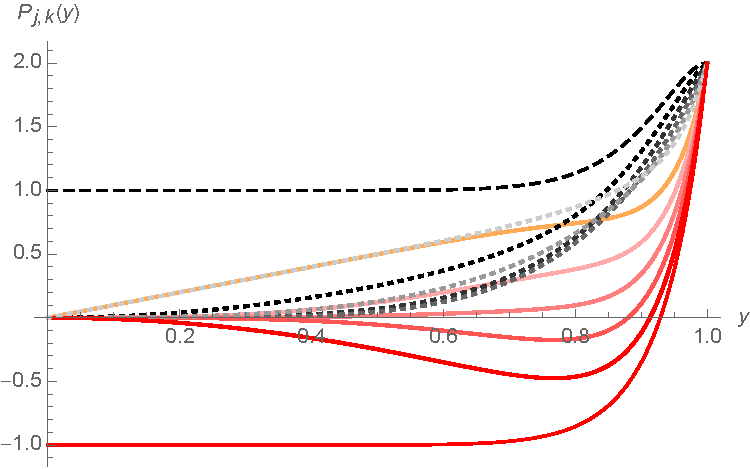
\includegraphics[width=0.5\textwidth]{fig_excepttopleft.pdf}
\caption{The polynomials in the first row of $M$, except for the top left polynomial. Even: black. Odd: red.}\label{fig_excepttopleft}
\end{center}
\end{figure}

\begin{figure}
\begin{center}
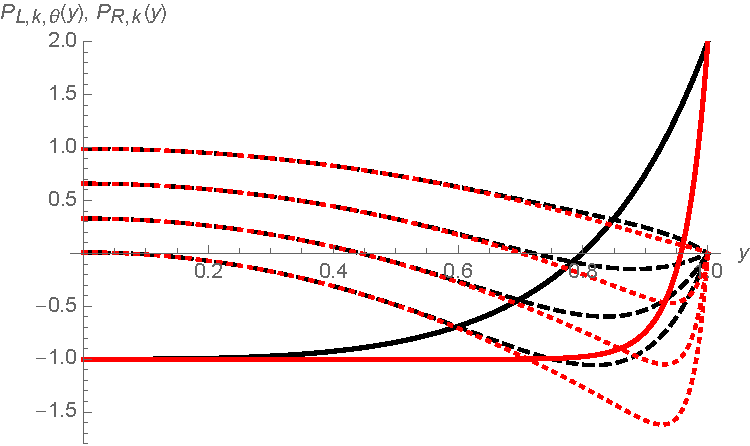
\includegraphics[width=0.5\textwidth]{fig_someplpr.pdf}
\caption{The red group ..., the black group .... Dotted red, solid red, dashed black, solid black curve.}\label{fig_someplpr}
\end{center}
\end{figure}

\begin{figure}
\begin{center}
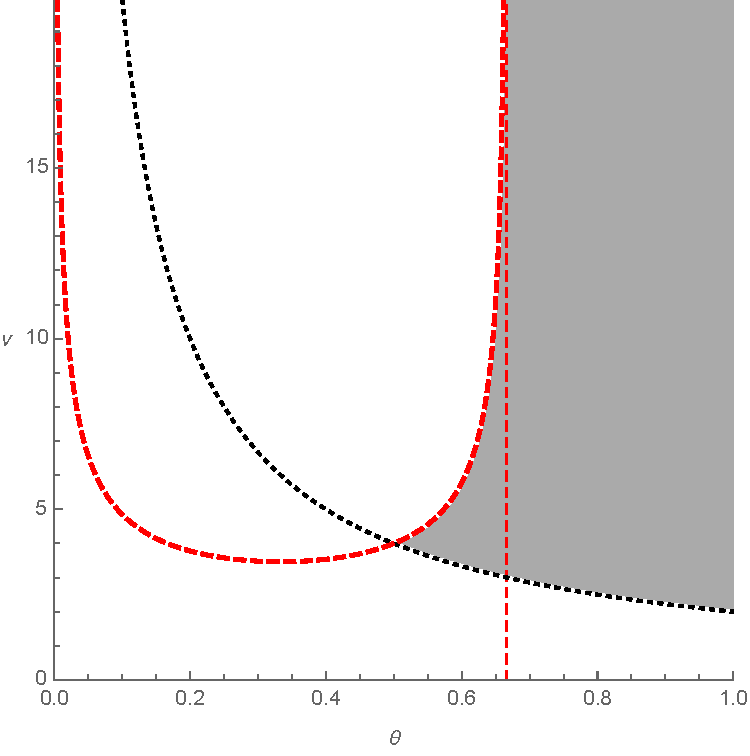
\includegraphics[width=0.48\textwidth]{fig_boundary.pdf}
\caption{Boundary curves for $m=3$ in the $(\te,\nu)$ parameter plane. The shaded region shows the parameter values in this window for which $M(3,\te,\nu)\ge 0$.}\label{fig_boundary}
\end{center}
\end{figure}

... about the non-negativity of the top left, and the top right entries of $M$.
\begin{lemma}
For any $k\in\nplus$ and $\te\in(0,1]$ we have 
\[
M_{1,1}(2k+1,\te,\nu)\ge 0 \quad \Longleftrightarrow \quad \nu\le\nul
\] 
and
\[
M_{1,2k+1}(2k+1,\te,\nu)\ge 0 \quad \Longleftrightarrow \quad \nu\ge\nur.
\] 
\end{lemma}
\begin{proof}
\end{proof}



... a necessary and sufficient condition for the non-negativity of the matrix $M$ for odd sizes.
\begin{lemma}
For any $k\in\nplus$ and $\te\in(0,1]$ we have 
\[
M(2k+1,\te,\nu)\ge 0 \quad \Longleftrightarrow \quad \nur\le\nu\le\nul.
\] 
\end{lemma}
\begin{proof}
\end{proof}


... to explain Figure \ref{fig_variousk} we use the following result.
\begin{lemma}
For any $k\in\nplus$ and $\te\in\left(0,\frac{1}{2}\right)$ we have 
\[
 \nur>\nul.
\] 
\end{lemma}
\begin{proof}
\end{proof}

\begin{theorem}
DESCRIBING $M(2k+1,\te,\nu)\ge 0 $ FOR FIXED VALUES OF $\te$.
DIFFERENT CASES TO MENTION:
$\te=0$ (the explicit Euler method), $0<\te<1/2$, $\te=1/2$ (second order method), $1/2<\te<1$, $\te=1$ (the implicit Euler method). FINITELY MANY $k$ VALUES.
\end{theorem}

\begin{remark}
ABOUT THE SIGN PATTERN OF THE MATRICES CORRESPONDING TO CORNER POINTS OF THE DIAGRAM
\end{remark}


\begin{lemma}
SOME ASYMPTOTIC PROPERTIES OF $\nu_R(k,1)$.
\end{lemma}



\subsection{Structured non-negative inverse eigenvalue problems}

Due to the fact that the eigenvalues of the matrix $M$ in \eqref{Mdef} are known, we can use some necessary conditions... Perron--Frobenius theorem, $\lambda_1$ non-negative real dominant root. 
It turns out that these general theorem restrict the parameter values. We give the following example.

Let us consider the $\te=1$ case. ...
These  can obtain (some weaker, why?) information on the para size of the entries $M_{i,j}$.

\section{Other discretizations}

\end{document}
